\chapter{Introduction} \label{cpt:Introduction}

\section{Abstract}

This report discusses the development of the R package \mintinline{R}{rmcop}, an fully R-based package for pricing financial options (see Section \ref{sec:Literature Review} for definitions). Pricing financial options is an essensial fragment of financial engineering and quantitative finance. Because options consider future in time, determining their fair price involves modelling uncertainty, so statistical methods are widely applied. Modern option pricing methods can be complex and product-specific, but most works are still built upon the basic frameworks of Black-Scholes formula and Monte Carlo simulations. The package \mintinline{R}{rmcop} covers the R implementation of some of these fundamental option price models on various option types and styles, and can be a good reference for constructing more complex R opiton pricing algorithms.

\section{Report Structure}

Here in Chapter \ref{cpt:Introduction}, the literature review in Section \ref{sec:Literature Review} will introduce necessary definitions of financial options and option pricing methods that are included in \mintinline{R}|rmcop| package. This is accompanyed by some useful formula deductions that will be seen useful in Chapter \ref{cpt:Pkg Dev}, where we will discuss the programming implementation of these models.

In Chapter \ref{cpt:Existing Packages}, we will introduce three existing option pricing packages in R (\mintinline{R}|derivmkts|, \mintinline{R}|fOptions|, \mintinline{R}|RQuantLib|), and explain their functionalities. We will also discuss their advantages and limitations.

In Chapter \ref{cpt:Pkg Dev}, we will discuss the package structure of \mintinline{R}|rmcop|. This includes: 1. a discussion on R's generic Objective Oriented Programming (OOP) environment; 2. an outline of the package's structure; and 3. a detailed elaboration of the R implementation techniques of the financial models introduced in Section \ref{sec:Literature Review}.

Finally in Chapter \ref{cpt:Results}, we will demonstrate examples and interpretations using \mintinline{R}|rmcop|. The report is then concluded by a discussion on \mintinline{R}|rmcop|'s limitations and plans for further development.

\section{Package Description} \label{sec:Pkg Description}

\mintinline{R}|rmcop| is an R package used for pricing financial options. The name ``rmcop'' stands for ``R Monte Carlo Option Pricing''. The package supports Monte Carlo based pricing for European vanilla options and European exotic options, including Asian, Barrier, Binary, and Lookback options. It also provides some deterministic methods for both European and American vanilla options pricing, including option pricing via Binomial lattice tree and Black-Scholes formula.

Unlike most existing packages in the R Ecosystem, \mintinline{R}|rmcop| is developed through an object oriented approach. User's argument inputs for pricing functions are encapsulated in corresponding objects, and pricing functions are themselves methods. This introduces ordered arguments control and easier functions application.

\section{Machine Environment}

The majority of the development and testing of the package is completed using my laptop. The machine is an Honor MagicBook Pro 2020, with AMD R7-4800H CPU which has 8 cores and 16 strands.

\section{Literature Review} \label{sec:Literature Review}

\subsection{Pricing of Financial Options}

An option is a common financial derivative\footnote{a security whose value depends on an the value of an underlying (i.e. the related) asset.} in the market. Options can be roughly classified into two types, ``call'' or ``put''. A call option, ``gives its holder the right (but not the obligation) to purchase from the issuer a prescribed asset\footnote{Underlying asset/stock, the word "asset" and "stock" may be used interchangably through this report.} for a prescribed price (strike price) at a prescribed time (maturity / expiration) in the future.\cite{Higham2004}'' Similarly, a put option gives the right to sell.

The two most common styles of financial options are European options and American options. An European option can only be exercised at maturity, whereas an American option can be exercised at anytime prior to maturity (which is a more complex setting).

The most typical "family" of options are the so called ``vanilla options'', which includes no special or unusual features seen in exotic options (see list below). For vanilla cases, an European call option has a payoff of $(S_T-K)^+ \coloneqq \max{(S_T-K,0)}$, and an European put option has a payoff of $(K-S_T)^+ \coloneqq \max{(K-S_T,0)}$ \cite{Glasserman2003} at the point of exercise $T$ (i.e. maturity). Here, $S_t$ is the underlying asset price at time $t\in[0,T]$, and $K$ is the option's strike price.

Options with ``special or unusual features'' are called ``exotic options''. The exotic options whose pricing are supported by \mintinline{R}|rmcop| package are introduced below based on the definitions given in \textit{An Introduction to Financial Option Valuation} \cite{Higham2004}.

\begin{itemize} \label{lst:exotic_options}
    \item \textbf{Asian Options} Asian options' payoff are determined by the average price of the underlying asset throughout its life span.
    \begin{itemize}
		\item An average price Asian call option has payoff at the expiry $T$ given by $\max(\bar{S} - K)$.
		\item An average price Asian put option has payoff at the expiry $T$ given by $\max(K - \bar{S})$.
		\item An average strike Asian call option has payoff at the expiry $T$ given by $\max(S_T - \bar{S})$.
		\item An average strike Asian put option has payoff at the expiry $T$ given by $\max(\bar{S} - S_T)$.
	\end{itemize}
    \item \textbf{Barrier Options} Barrier options have a payoff that switches on or off depending on whether the asset crosses a pre-defined level (barrier) $B$.
    \begin{itemize}
		\item A down-and-out call option has a payoff that is zero if the asset crosses some predefined barrier $B<S_0$ at some time in $[0, T]$. If the barrier is not crossed then the payoff becomes that of a European call, $\max(S_T - K, 0)$.
		\item A down-and-in call option has a payoff that is zero unless the asset crosses some predefined barrier $B<S_0$ at some time in $[0, T]$. If the barrier is crossed then the payoff becomes that of a European call, $\max(S(T) - K, 0)$.
    \end{itemize}
    \item \textbf{Binary Options} A binary (a.k.a. cash-or-nothing) option have payoff at expiry being either some specified value $A$ or zero.
    \begin{itemize}
		\item A binary call option has payoff $A$ if $S_T>K$ and zero otherwise.
		\item A binary put option has payoff $A$ if $S_T<K$ and zero otherwise.
	\end{itemize}
    \item \textbf{Lookback Options} The payoff for a lookback option depends upon either the maximum $S^{\max}$ or the minimum value $S^{\min}$ attained by the asset throughout the price trajectory.
    \begin{itemize}
		\item A fixed strike lookback call option has payoff at expiry $T$ given by $\max(S^{\max}-K, 0)$.
		\item A fixed strike lookback put option has payoff at expiry $T$ given by $\max(K-S^{\min}, 0)$.
		\item A floating strike lookback call option has payoff at expiry $T$ given by $S_T -S^{\min}$.
		\item A floating strike lookback put option has payoff at expiry $T$ given by $S^{\max} -S_T$.
    \end{itemize}
\end{itemize}

\subsection{Brownian Motion}

A \textit{stochastic process}, by definition \cite{Iacus2008}, is a family of random variables $\{X_\gamma,\gamma\in\Gamma\}$ defined on $\Omega\times\Gamma$ taking values in $\mathbb{R}$. Thus, the random variables of the family (measurable for every $\gamma\in\Gamma$) are functions of the form:

\begin{align*}
X(\gamma,\omega):\Gamma\times\Omega\mapsto\mathbb{R}
\end{align*}

Where $(\omega,\mathcal{A},P)$ is a probability space described by samples $\omega$, action space $\mathcal{A}$, and probability measure $P$.

For $\Gamma=\mathbb{N}$, we have a \textit{discrete process}, and for $\Gamma\subset\mathbb{R}$, we have a \textit{continuous process}. In our context we will consider $\Gamma$ to represent the scope in time, and takes values from $0$ to option's maturity $T$.

A stochastic process $\{X(t), t\geq 0\}$ is said to be a \textit{Brownian motion} if \cite{Iacus2008}:

\begin{enumerate}
	\item $X(0)=0$;
	\item $\{X(t),t\geq0\}$ has stationary and independent increments.
	\item for every $t>0$, $X(t)\sim N(0,\sigma^2 t)$.
\end{enumerate}

\begin{figure}[H]
	\centering
	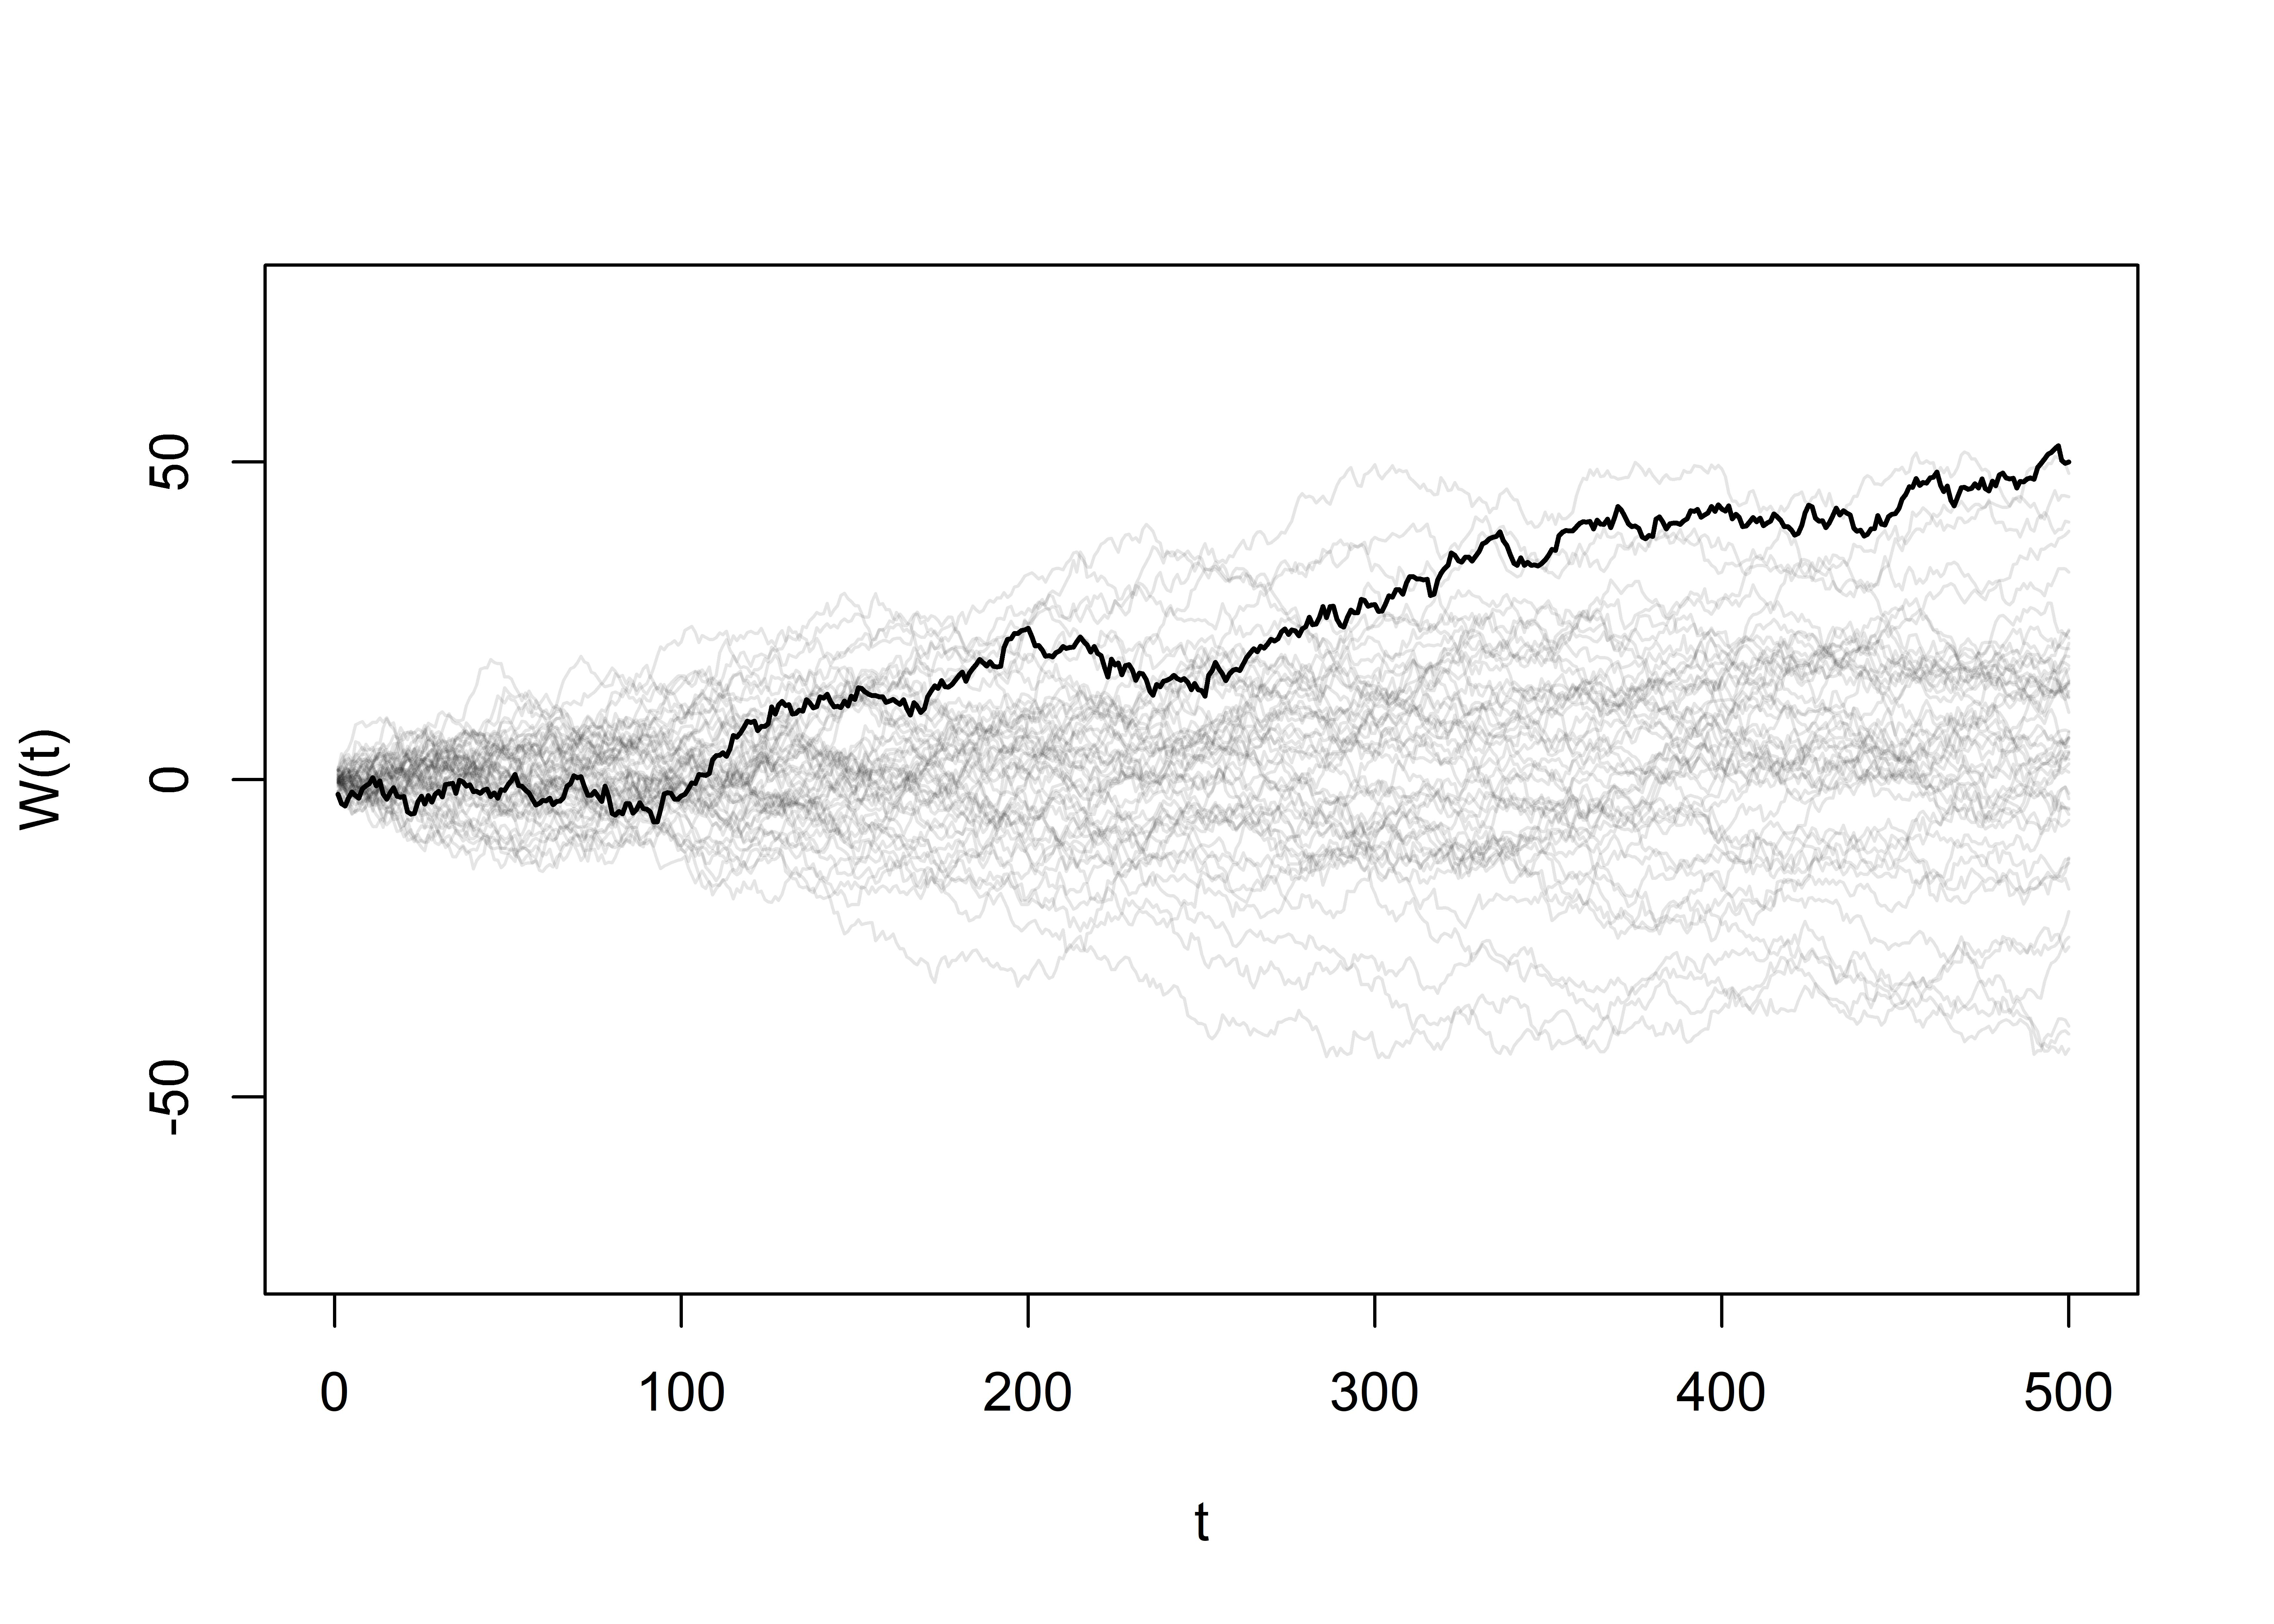
\includegraphics[scale = 0.5]{wiener_process.jpeg}
	\caption{Wiener Process} \label{img:wiener_process}
\end{figure}

Image \ref{img:wiener_process} demonstrates the trajectories of a one-dimensional Standard Brownian Motion (SBM, Wiener Process), where each gray line represents a simulated path of a Wiener process.

Notice that the expectation of a SBM at any time $t\geq0$ is zero, this makes the SBM a \textit{martingale}, which is a stochastic process that "does not tend to rise or fall \cite{Shreve2004}". If $S_t$ is the value of a SBM at time $t$, assume $S_0=0$, its SBM dynamics can be defined by the Stochastic Differential Equation (SDE):

\begin{align*}
dS_t = S_t dW_t
\end{align*}

We can generalised the scenarios by considering drifts through time (measured by $\mu$) and scaling the amount of diffusion with respect to time (measured by $\sigma$). For $S_t$ that follows a \textit{Geometric Brownian Motion} (GBM), its dynamics can be described by the SDE \cite{Shreve2004}:

\begin{align*}
dS_t = \mu S_t dt + \sigma S_t dW_t
\end{align*}

Where $\mu S_t dt$ is called the \textit{drift term} and $\sigma S_t dW_t$ the \textit{diffusion term}.

Expanding on $S_t$, for a function $f:\mathbb{R}\mapsto\mathbb{R}$, the GBM $f(S_t)$ is described as, according to Itô's rule \cite{Shreve2004}:

\begin{align*}
df(S_t) = \left[\mu_t\frac{\partial f}{\partial S}(S_t)+\frac{1}{2}\frac{\partial^2 f}{\partial S^2}(S_t)\right]dt + \sigma_t\frac{\partial f}{\partial S}dW_t
\end{align*}

Using Itô-Doeblin rule for $f:\mathbb{R}\mapsto\mathbb{R}$ \cite{Shreve2004}, we can derive the following explicit solution to the SDE:

\begin{align} \label{eq:GBM_explicit}
f(S_t) = f(S_0) + \int_{0}^{t}{\mu_t\frac{\partial f}{\partial S}(S_t)}dt + \frac{1}{2}\int_{0}^{t}{\sigma_t^2\frac{\partial^2 f}{\partial S^2}(S_t)}dt + \int_{0}^{t}{\sigma_t\frac{\partial f}{\partial S}(S_t)}dW_t
\end{align}

Equation \ref{eq:GBM_explicit} will be shown useful in the Black-Scholes model introduced in the following section.

\subsection{Black-Scholes Model}

The very first attempt of applying quantitative method in option pricing (perhaps in all finance) is by the French mathematician Louis Bachelier in 1900. In his work \textit{The Theory of Speculation} \cite{Bachelier1900}, he deducted deterministic formulas for pricing European (vanilla) call and put options as follows:

\begin{align*}
C(S, T) &= SN(\frac{S - X}{\sigma\sqrt{t}}) - XN(\frac{S - X}{\sigma \sqrt{t}}) + \sigma\sqrt{t}N(\frac{S - X}{\sigma \sqrt{t}}) \\
P(S, T) &= XN(\frac{S - X}{\sigma \sqrt{t}}) - SN(\frac{S - X}{\sigma \sqrt{t}}) + \sigma\sqrt{t}N(\frac{S - X}{\sigma \sqrt{t}})
\end{align*}

Being the earlist approach, Bachelier's formula had already outlined the relationship between option price and asset price $S$, strike price $X$, and volatility measure $\sigma$, which are essential fragments in modern formulas. However, based on limited data, Bachelier's solution was built under some unrealistic assumptions. The normality assumption violates the non-negativity of the stock price, and the formula's discrete measure in time omitted the effect of continuous movements in the stock price. Also, the formula did not discount the effect of interest rate. These errors cause Bachelier's model fails to price options accurately.

It wasn't until 1960s had further improvement been made to quantitative option pricing. In 1961, Case Sprenkle \cite{Sprenkle1961} introduced the Sprenkle formula. The formula addressed the above issues by describing the stock price by the more suitable log-normal distribution and discounting for the effect of interest rate, which successfully explained the time value of an option. In the following decade, improvements have been made by scholars such as Boness and Samuelson \cite{BS1973}, who introduced emperical constants to increase the effectiveness of Sprenkle's model.

The model was finalised by Black and Scholes in 1973 \cite{BS1973}, who explained the stock price movement by GBM. The GBM was described in the form of a Stochastic Differential Equation (SDE), which effectly model the continuity of price movement. The solution (derived through Itô's lemma) of Black-Scholes formula under an risk-neutral approach\footnote{The risk-neutral approach, in simple terms, is constructing a portfolio at a moment in time such that the portfolio value will be identical at the next moment in time regardless of the price movement, so the portfolio will be riskless to the price movement.} eliminates the emperical measure of Sprenkle et al's model, which resulted in an objective and deterministic estimation of option price, as is used by most contemporary pricing methods.

Recall the explicit form of an SDE $f(S_t)$ given by Itô-Doeblin rule in Equation \ref{eq:GBM_explicit}. We assign $f(S_t)=\log(S_t)$ where $\log$ is the natural logarithm. The solution is:

\begin{align} \label{eq:BS_log_explicit}
\log(S_t) = \log(S_t) + (\mu - \frac{\sigma^2}{2})t + \sigma W_t
\end{align}

Because $W_t\sim N(0, t)$, we can see that Equation \ref{eq:BS_log_explicit} shows that:

\begin{align*}
\log(S_t)\sim N(\log(S_0)+(\mu - \frac{\sigma^2}{2})t, \sigma^2 t)
\end{align*}

This implies that $S_t$ follows a \textit{log-normal} distribution. A log-normal distribution takes only positive value, which addressed the negativity issue caused by Gaussian stock price models, like the one developed by Bachelier \cite{Bachelier1900}.

By taking the exponential on the two sides of the equation, one can obtain the following expression:

\begin{align} \label{eq:BS_explicit}
S_t = S_0\exp{\left\{(\mu-\frac{\sigma^2}{2})t + \sigma W_t\right\}}
\end{align}

Which describes the stock price $S_t$ at anytime $t\in[0,T]$. When simulating real market conditions, one may replace the factor $\mu$ with $r$ and $q$, which stands for the (fixed) interest rate and dividend yield rate, respectively.

\begin{align*}
S_t = S_0\exp{\left\{(r-q-\frac{\sigma^2}{2})t + \sigma W_t\right\}}
\end{align*}

Under the risk-neutral assumption, the payoff of a (European vanilla) call option with strike price $K$ and expiration $T$ is given by the expectation $E[e^{-rT}(S(T)-K)^+]$, and the corresponding payoff of a (European vanilla) put option at the same strike price and expiration is given by $E[e^{-rT}(K-S(T))^+]$. Using the solution of the Black-Scholes SDE we can deterministically eavluate the payoffs as follows \cite{Higham2004}:

\begin{align*}
&C(S(0), T) = S(0)\Phi(d_1) - e^{-rT}K\Phi(d_2) \\ 
&P(S(0), T) = e^{-rT}K\Phi(-d_2) - S(0)\Phi(-d_1)
\end{align*}

Where $\Phi$ is the cumulative normal distribution, $d_1 \coloneqq \frac{\log(S(0)/K)+(r+\frac{1}{2}\sigma^2)T}{\sigma\sqrt{T}}$, and $d_2 = d_1 - \sigma\sqrt{T}$. The Equations \ref{eq:BS Formula Call} and \ref{eq:BS Formula Put} are the so-called Black-Scholes formula.

A genearlised solution which addressed the impact of the presence of dividends (assuming the option of interest has an annual dividend yield rate of $\delta$) specified as \cite{Glasserman2003}:

\begin{align}
	&C(S(0), T) = e^{-\delta t}S(0)\Phi(d_1) - e^{-rT}K\Phi(d_2) \label{eq:BS Formula Call} \\
	&P(S(0), T) = e^{-rT}K\Phi(-d_2) - e^{-\delta t}S(0)S(0)\Phi(-d_1) \label{eq:BS Formula Put}
\end{align}

Where now $d_1 \coloneqq \frac{\log(S(0)/K)+(r-\delta+\frac{1}{2}\sigma^2)T}{\sigma\sqrt{T}}$.

A further result to the American option cases is such that an American call option is never optimal (i.e. the estimated value would be the same as the European call option under same conditions), and that an American put option's value does not have an analytical form and required numerical methods to calculate\footnote{This is related to the studies on Monte Carlo pricing for American Options, which is beyond the current scope of \mintinline{R}|rmcop|.}.

\subsection{Binomial Lattice Model}

In 1979, based on the risk-neutral approach used by the Black-Scholes model, Cox, Ross and Rubinstein (CRR) \cite{CRR1979} introduced a Binomial lattice tree model for modelling stock prices.

To construct a Binomial tree of stock prices, one breaks down the option's life $[0,T]$ into $n$ time steps with fixed interval $\Delta t=T/n$. For each time steps, the stock price can move either up by a factor $u$ with probablity $\hat{p}$ or down by a factor $d$ with probability $\hat{q}=1-\hat{p}$.

\begin{figure}[H]
    \centering
    \[\tikz{
        \node (a) at (0, 2) {$S$};
        \node (b) at (2.5, 3) {$uS$};
        \node (c) at (2.5, 1) {$dS$};
		\node (d) at (5, 4) {$u^2S$};
        \node (e) at (5, 2) {$udS$};
		\node (f) at (5, 0) {$d^2S$};
        \path[->] (a) edge node [above left] {$\hat{p}$} (b)
				  (a) edge node [below left] {$1-\hat{p}$} (c);
		\path[->] (b) edge node [above left] {$\hat{p}$} (d)
        		  (b) edge node [above right] {$1-\hat{p}$} (e);
		\path[->] (c) edge node [below right] {$\hat{p}$} (e)
        		  (c) edge node [below left] {$1-\hat{p}$} (f);
    }\]
    \caption{Binomial Lattice Tree for Stock Price with 2 Steps} \label{gph:binomial_tree}
\end{figure}

As Figure \ref{gph:binomial_tree} shows, we will obtain a total of $n+1$ nodes at maturity $T$. For each node at the final step, we can obtain the corresponding payoff of an option related to that stock price. For example, recall from the above section, the $n+1$ possible payoffs $P(S(T))$ of an vanilla European call option would be:

\begin{align}
P(S(T))=(S(T)-K)^+
\end{align}

The probability $\hat{p}$ is set to be ``risk neutral'' in a way such that:

\begin{align}
S(t_{i}) &= e^{-r\Delta t}\mathbb{E}[S(t_{i+1})] \\
		 &= e^{-r\Delta t}[\hat{p}uS(t_i)+\hat{q}dS(t_i)],\quad\text{for }i=0,...,n-1
\end{align}

Meaning that the current node's stock price is equal to the expected value of the two future nodes it can go in the next time step, discounting the interest. In such way, a portfolio which consist only of this stock would have a fixed return under price movement.

Under such setting, the option payoff at each node is computed in similar way. Suppose payoff $P_{ij}$ denotes the payoff of the $j$th node at time step $i$, it can be computed via recursive form:

\begin{align}
P_{ij} &= e^{-rT}[\hat{p}P_{(i+1),j+1} + \hat{q}P_{(i+1),j}]
\end{align}

As mentioned above, the payoff of an option at maturity $T$ is obvious to obtain. By applying this recursive method forward from $t=T$ back to $t=0$, we will obtain an deterministic estimate of the current payoff (fair value) of the option of interest.

\subsection{Monte Carlo Option Pricing}

As the financial market develops and more complicated options emerge, in many realistic cases, one cannot find a deterministic solution for pricing option. However, thanks to the advancement of computer power, one can simulate price trajectories for enormous times, and estimate the payoff of the option of interest by simply taking the average of the option payoff under each simulated trajectory. Such method is known as the Monte Carlo method. The very first attempt of applying computational method in option pricing is by Phelim Boyle in 1977. More serious (and effective) approach was introduced by Paul Glasserman in the 1990s based on the Black-Scholes model. Until now, the field of Monte Carlo option pricing is still under active development and is widely used by "quants". The contents below will elaborate implementation method as the one introduced in Glasserman's \textit{Monte Carlo Methods in Financial Engineering} \cite{Glasserman2003}.

We know that a GBM is a continuous process, and its dynamics is described by an SDE with respect to the $t$ through infinitesimal $dt$. In order to simulate the process, we need to discretise $dt$ to the computable $\Delta t$.

Recall the explicit form of the GBM (Equation \ref{eq:BS_explicit}) introduced in the Black-Scholes model, we can expand on it to describe the change in asset price $S_{t+\Delta t}$ as:

\begin{align*}
S_{t+\Delta t} = S_t\exp{\left\{(\mu-\frac{\sigma^2}{2})\Delta t+\sigma W_{\Delta t}\right\}}
\end{align*}

Knowing that $W_t\sim N(0,t)$, suppose we have $Z\colonsim N(0,1)$, we have $W_t=Z\sqrt{t}$. So we can modify the above equation to:

\begin{align*}
S_{t+\Delta t} = S_t\exp{\left\{(\mu-\frac{\sigma^2}{2})\Delta t+\sigma Z \sqrt{\Delta t}\right\}}
\end{align*}

Suppose we discretise the continuous time interval $[0,T]$ into $m$ time steps with fixed length $\Delta t=\frac{T}{m}$. We can derive the iterative formula:

\begin{align} \label{eq:mc_explicit}
S_{i} = S_{i-1}\exp{\left\{(\mu-\frac{\sigma^2}{2})\Delta t+\sigma Z_i \sqrt{\Delta t}\right\}},\qquad i=1,...,m
\end{align}

We can also modify the equation to address the effect of interest rate and dividend yield rate according to what's mentioned below Equation \ref{eq:BS_explicit}:

\begin{align} \label{eq:mc_explicit_rq}
S_{i} = S_{i-1}\exp{\left\{(r-q-\frac{\sigma^2}{2})\Delta t+\sigma Z_i \sqrt{\Delta t}\right\}},\qquad i=1,...,m
\end{align}

By simulating $m$ standard normal random variables $Z_1,...,Z_m$, we will be able to generate a full trajectory of the price movements.

\begin{algorithmic}
\For{$i \gets 1,...,m$}
	\State $Z_{i} \gets N(0,1)$
	\State $S_{i} \gets S_{i-1}\exp{\left\{(\mu-\frac{\sigma^2}{2})\Delta t+\sigma Z_i \sqrt{\Delta t}\right\}}$
\EndFor
\end{algorithmic}

Noticing that as $W_T\sim N(0,T)$, and that individual increments for Brownian motions are independent, the approximation of $W_T$ using $Z_i$'s is lossless (i.e. the number of time steps / length of $\Delta t$, has no effect on how well the approximation will be). For path-independent options\footnote{Options whose payoff only depends on the stock price at maturity, $S_T$.}, it may be wise to take $m=1$, i.e. $\Delta t=T$ to minimise the computational cost.

If we are to simulate $n$ times, for the $i$th trajectory, $i=1,...,n$, one may employ formulas introduced in List \ref{lst:exotic_options} and discounting the effect of interest rate and dividend rate to obtain the corresponding discounted payoff (i.e. fair price) of the option, $C_i$. For example, the discounted payoff of an Vanilla call option, at maturity, can be calculated as:

\begin{align} \label{eq:discount_vanilla_payoff}
C_i = e^{-rT}(S_T-K)^+
\end{align}

The Monte Carlo estimator for the option price is then simply the arithmetic mean $\hat{C}_n\coloneqq\frac{1}{n}\sum_{i=1}^{n}{C_i}$. This estimator is \textit{unbiased} and \textit{strongly consistent} \cite{Glasserman2003}.

For large enough $n$, we can construct a confidence interval using the standard error, given by \cite{Glasserman2003}:

\begin{align} \label{eq:mc_SE}
SE_C &= \frac{s_C}{\sqrt{n}} \\
 s_C &= \sqrt{\frac{1}{n-1}\sum_{i=1}^{n}{(C_i-\hat{C}_n)^2}}
\end{align}

Glasserman in his work \cite{Glasserman2003} also indicated the criterion for the simulation estimators' efficiency: computing time, bias, and variance. The estimators considered in our package are unbiased, and variance reduction techniques are beyond our scope. So we will only discuss some R programming methods in reducing the computing time to increase estimation efficiency, as we will see in Chapter \ref{cpt:Pkg Dev}.

\newpage